\begin{itemize}
	\item NHTSB says AV software is considered a driver. How does one bound the risk posed to society by software agent. 
	\item Driver's license is a set of tests, we attempt to generalize human behavior based on tests
	\item AV's don't necessarily fail in predictable ways, tests cover an infitesimal portion of the state space, need to gain confidence that algorithms are sound.
\end{itemize}
CPS perspective is an integrated approach that captures the manifestation of errors in the physical world. At its heart is the use of formal models of system and precise mathematical specifications of desired behavior. We are interested in developing the appropriate formal models, a set of specifications, and a battery of scenarios. The community needs to investigate how such methods scale, or fail to scale, and provide new solutions.

 \section{Verification of Autonomous Vehicle Planning}
 
 \subsection{How do you give a self-driving car a driver's license?}
 Each year there are an average of 1.24 million traffic fatalities around the world \cite{Waldrop2015}. Estimates indicate that more than 90 percent of all accidents are due to driver error \cite{Waldrop2015}. Competent autonomous vehicles (AVs) could drastically reduce the occurrence of such incidents, but a major question first needs be answered:
 how can we judge when an AV is ready to graduate from research laboratories to public roads?
 One thing is clear: the public will want significant evidence that AVs are indeed safe \cite{weld1994first}. 
 This raises significant ethical and legal questions about how the AV should behave, and technical questions about how to \emph{verify} that it will always behave the way its designers intended.
 
 Prototype AVs have driven millions of miles and are even being approved for \emph{testing} on public roads in some states \cite{Iozzio2014}; however, manufacturers cannot \emph{verify} (i.e., guarantee) the safety of even the simplest of scenarios in the presence of other dynamic traffic participants. 
 Compounding the difficultly of vehicle certification, vehicle manufacturers such as Tesla are transitioning to frequent over-the-air software updates. Such practice eschews conventional vehicle development technique and greatly increases pressure on developers to deliver correct software at a rapid pace. 
 
 The net result of the growing pressure to release AVs is a wide gap between current regulations and our technological capabilities. 
 Human drivers are not `certified' to act safely in all situations, in fact, we know they don't; however, they assume liability for their actions.
 Who is liable for the behavior of an AV? The manufacturer or the vehicle owner?
 Currently, it appears that manufacturers will take one of two approaches: (1) assume liability for the actions of the vehicle and self-insure \cite{volvo15Liability} or (2) force the human occupants of an AV to make all critical decisions and shift liability to the pilot \cite{maurer2015autonomes}. In either case, even if AVs reduce accidents by 99 percent, it is likely that the 1 percent of remaining accidents will invariably spawn a myriad of legal actions against \emph{both} manufacturers \cite{russell2015research} and vehicle owners.   
 If the legal question is not answered, these risks could stifle the development of the AV market.
 
 Thus, regardless of where legal liability falls it is clear that we first need new, practical methods for verification and validation of the decision engines of each AV.
 Furthermore, verification must be automatic, exhaustive, and expedient for clearly defined scenarios. 
 Secondly, ethical considerations still underlie both the design and verification of AVs: how does the safety of the car's passengers weigh against that of people in its environment? 
 Whose morals are embedded in the decision engines of an AV?
 
 \subsection{New and Old Challenges}
 
 Some of the problems facing would-be AV manufacturers in 2016 are very different than those outlined by the teams in the DARPA Urban Challenge \cite{buehler2009darpa}. One problem highlighted by the first ever crash between AVs at the Urban Challenge \cite{fletcher2008cornell} is that there are no known \quotes{formal methods that would allow definitive statements about the completeness or correctness of a vehicle interacting with a static environment, much less a dynamic one} \cite{urmson2008autonomous}.  Today one must still consider the massive configuration space of each individual snapshot of the day-to-day life of an AV if verification is to be attempted. For example, in order to test the interaction between two 7 DOF AVs requires $10^{14}$ simulations for only 10 samples from each state. If each test takes 10 seconds, the resulting set of simulations will take \emph{30 million years} to complete. Furthermore, within a given scenario, errors in localization, sensing, and actuation imply we never know the state of the world exactly. Small state estimation errors can befuddle motion planning algorithms and mean a difference between collision and safety in tight spots. As many teams in the Urban Challenge noted, a means of verifying the safety of autonomous driving is paramount to putting self-driving cars in the hands of the public \cite{urmson2008autonomous}. 
 
 In contrast to the Urban Challenge in 2007, in which only 6 teams out of an original 89 applicants were able to finish, many research labs find themselves in the position of being able to construct a convincing AV in a matter of months; such a vehicle might be relatively competent in 75 percent of the situations it faces, but the long tail of special cases beckons. In fact Sebastian Thrun, a veteran of Google's Self Driving Car project and the Urban Challenge, notes that \emph{there were many more of unusual situations than we believed in the beginning}. One possible solution to handling rare events and scenarios is to record such occurrences using consumer vehicles driving in real traffic; with each new scenario existing behavioral planners can be adjusted via a reinforcement learning scheme \cite{wei2013autonomous, Silver_2010, Waldrop2015}. Just as in the more vanilla scenarios, timely updates to controllers provided on the basis of a single example will need to be verified offline, before shipping, and without the thousands of miles of testing necessary for a typical safety feature. 
 
 \begin{figure}
 	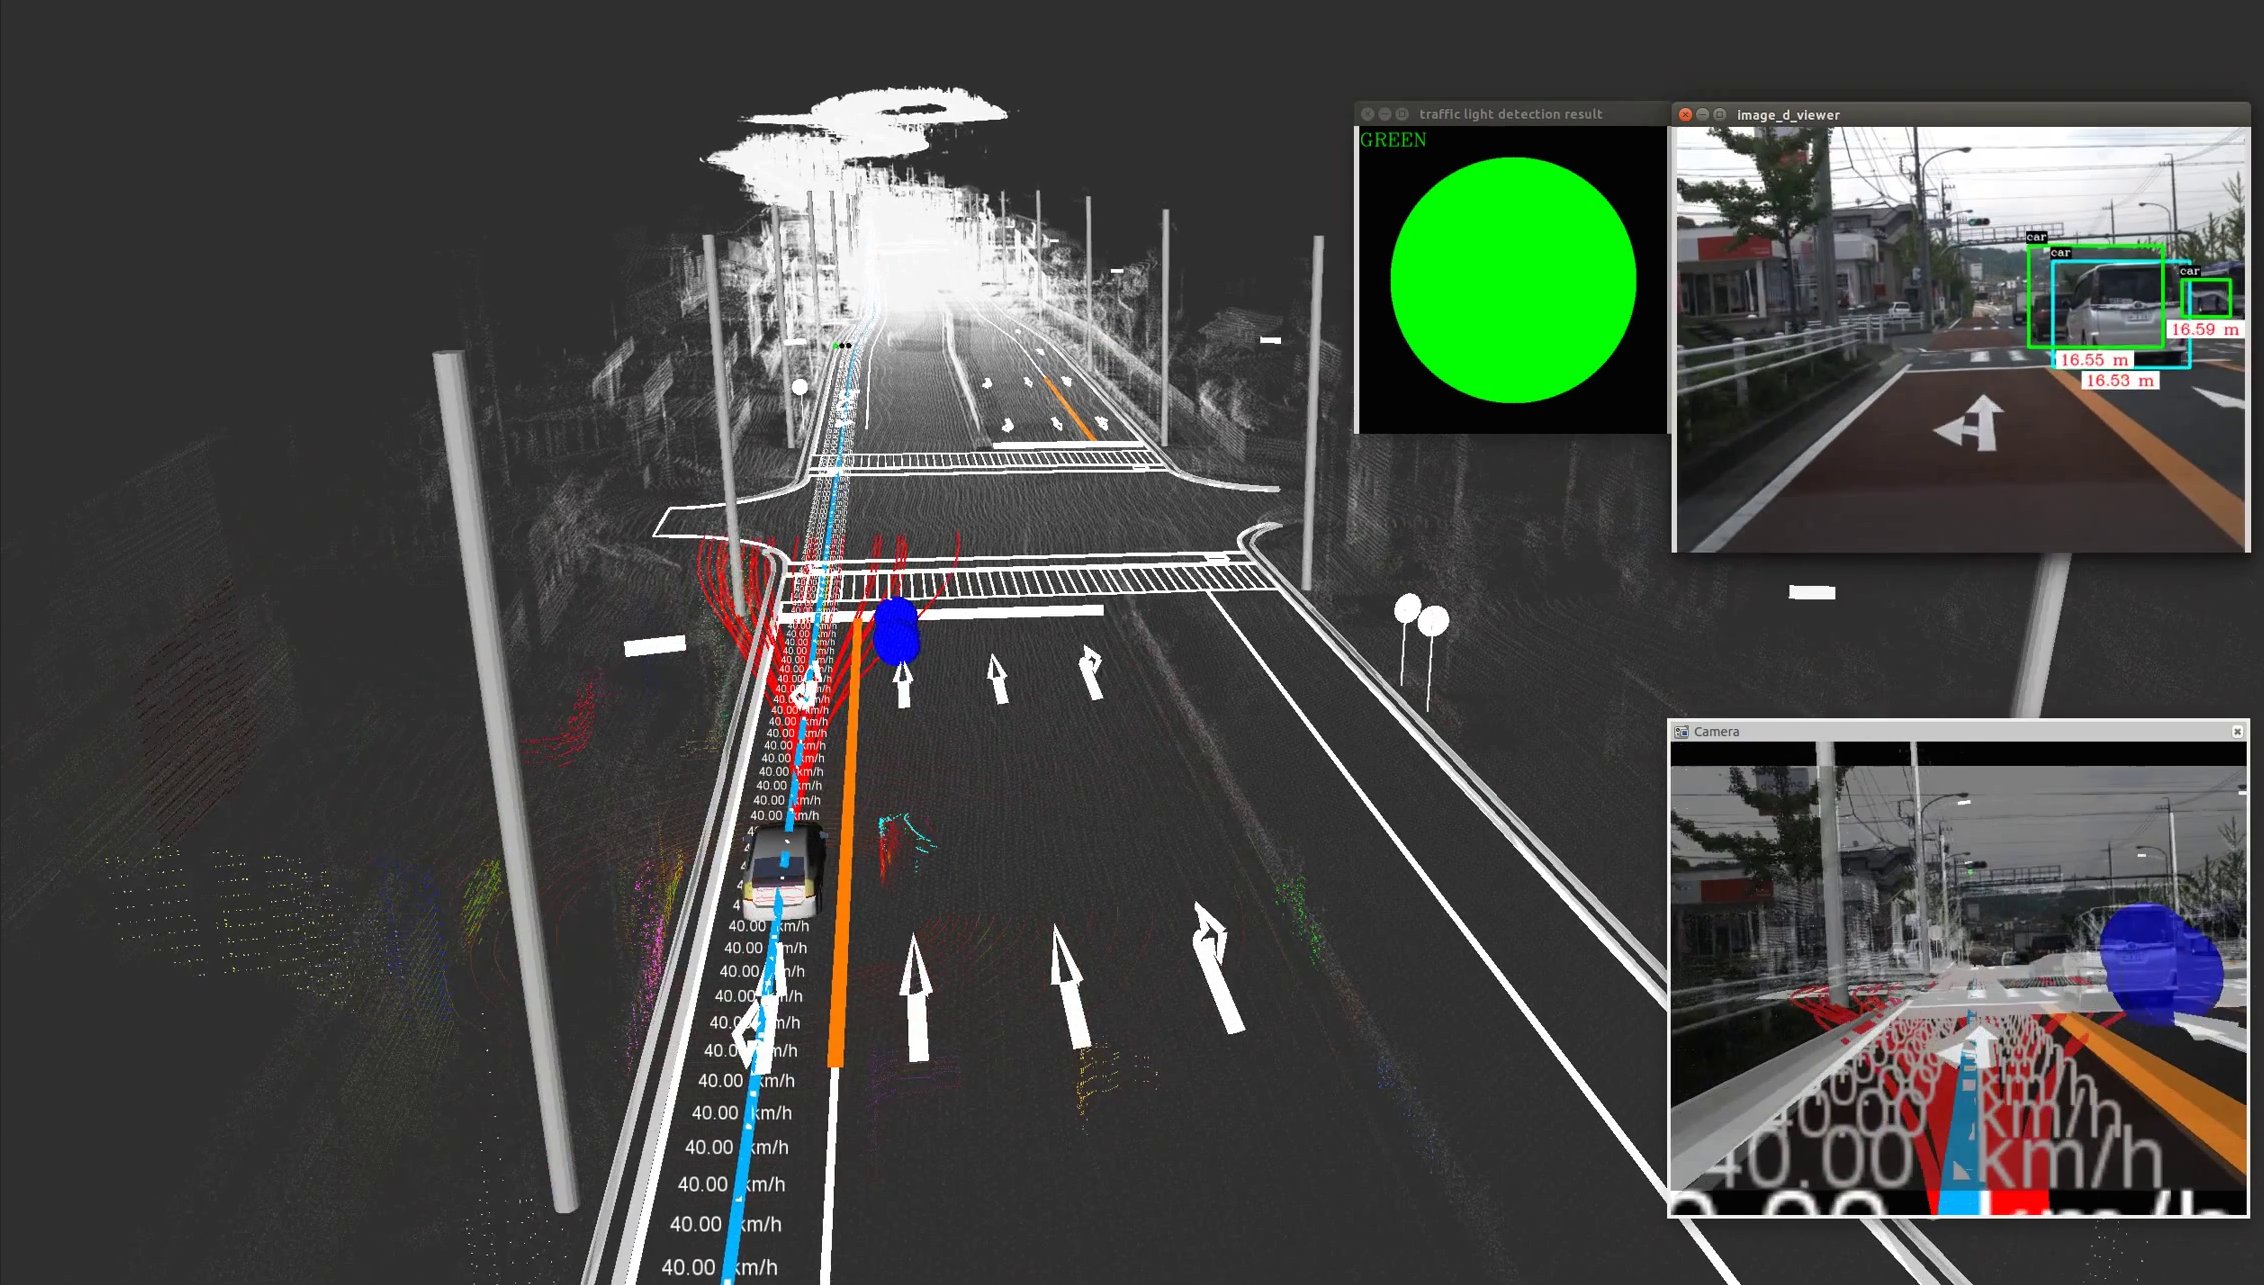
\includegraphics[width=\columnwidth]{figures/apex_planning.png}
 	\caption{Autonomous vehicle}
 \end{figure}
 
 
 %As Brian Soublet of the California DMV pointed out, he knows how to test a 16-year-old's driving skills, but he can't say the same for a car. At the same time, these regulators know that when a death inevitably happens—no amount of %self-driving cars will reduce annual road deaths to zero—they'll be attacked for allowing unsafe vehicles on the road.
 
 
 \subsection{The APEX approach}
 The APEX tool represents a new approach to solving both the problems of the Urban Challenge and investigating rare events encountered only through on road driving and testing. Unlike other tools capable of verifying controllers for hybrid systems we require almost no abstraction. Most current approaches look at only the behavioral layer and assume perfect implementation of plans at the motion planning layer. Instead, we propose that the behavioral layer is used to generate sequences of problems to be investigated at the level of motion planning and trajectory tracking.  Thus, APEX addresses the safety verification issue by leveraging new results in hybrid systems and reachability analysis \cite{gao2013satisfiability} to convert a brute force search over real intervals (which is intractable) into a set of finite sequences of bounded reachability problems. 
 \begin{figure}
 	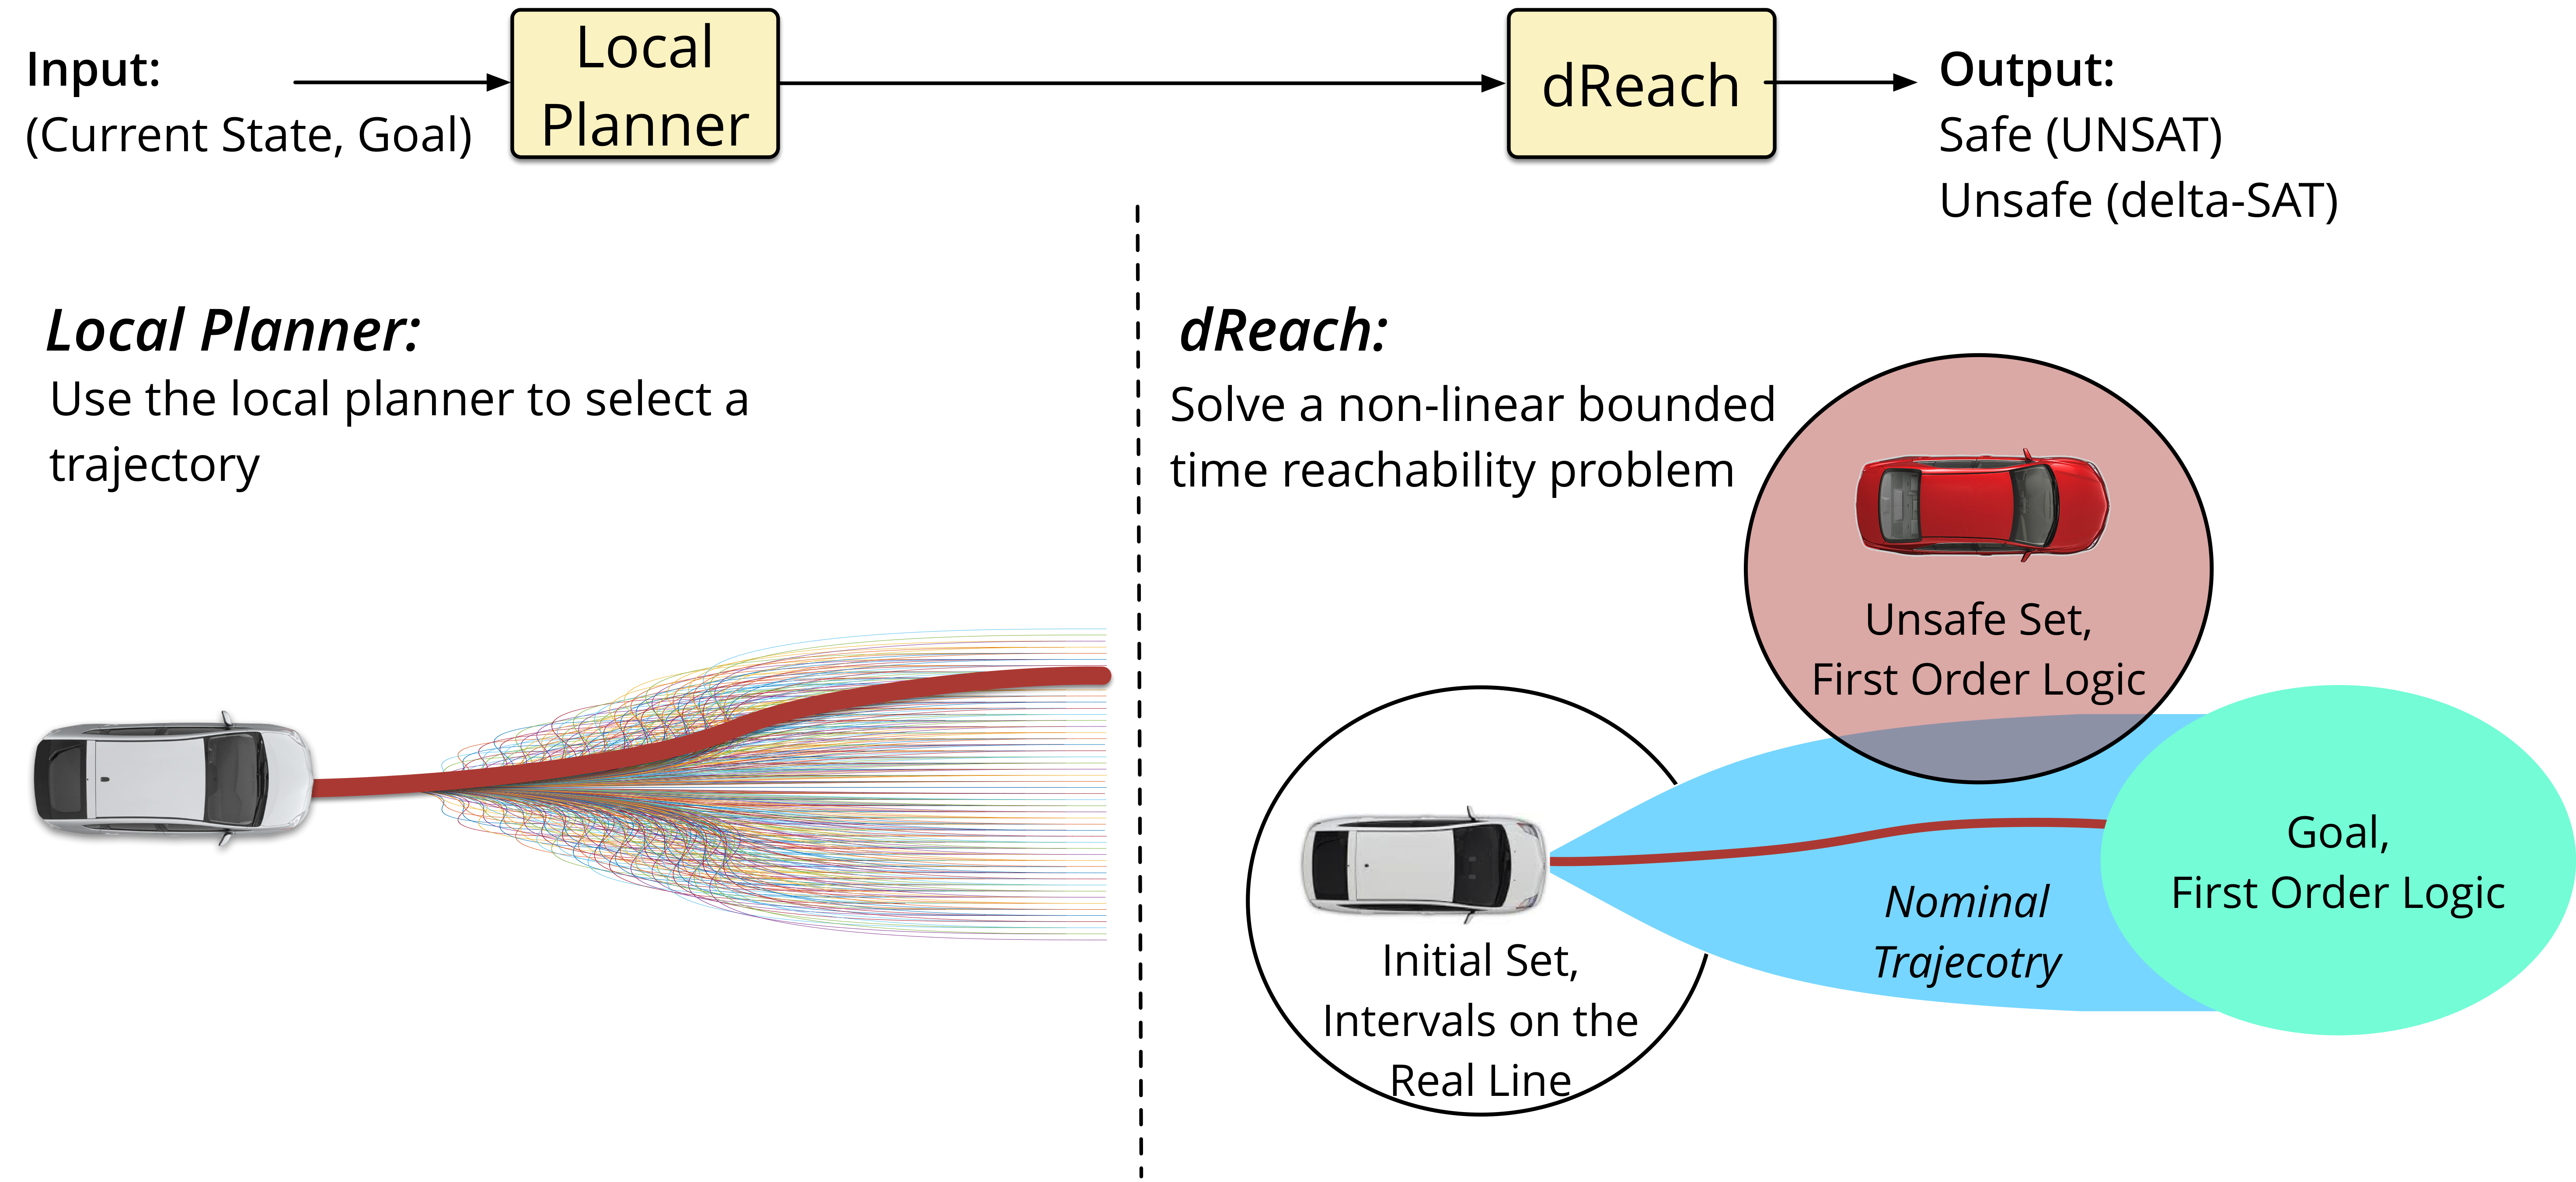
\includegraphics[width=\columnwidth]{Figures/tool_single}
 	\caption{A single offline execution of the APEX tool calls the local planner associated with the AV in order to generate a reachability problem}
 \end{figure}
 
 Using APEX we capture the output of trajectory generation and optimization based methods outside of the formal model of the system. Using such information, we generate a sequence of verification problems by running the through realistic vehicle dynamics and low level controls. The software which runs on the vehicle is used directly for verification. If a rare event is encountered and recorded by a real vehicle and a new rule or controller is added to the AV it is imperative that the manufacturer have high confidence that the modification will not induce new errors which are not evident in a single trace. APEX can make the most of rare events and scenarios; given a template we could find every possible instantiation and prove it is impossible for solution to make a decision leading to crash. The key features of our approach are:
 \begin{itemize}
 	\item Use of realistic planning software which runs on actual vehicles.
 	\item Modular vehicle model construction which can easily be replaced when new algorithms or alternate vehicle dynamics are necessary.
 	\item Non-conservative evaluation of safety and liveness at the level of the ego-vehicles actual spatial-temporal evolution. 
 \end{itemize}
 
 Thus, verification of realistic scenarios under all possible configurations over a length of 30-60 seconds is entirely feasible. Using such an approach a manufacturer, regulator, or insurer can begin to build a library of scenarios on which to test new vehicle software or updates made to the behavioral layer made through a reinforcement learner.
 
 \subsection{Future Work: verification, learning, ethics, and control}
 
 %In the literature on robot ethics, it remains arguable whether artificial agents without free
 %will can truly exhibit moral behavior [1]. However, it seems certain that other road users
 %and society will interpret the actions of automated vehicles and the priorities placed by their
 %programmers through an ethical lens. Whether in a court of law or the court of public opinion,
 %the control algorithms that determine the actions of automated vehicles will be subject
 %to close scrutiny after the fact if they result in injury or damage. In a less dramatic, if no
 %less important, manner, the way these vehicles move through the social interactions that
 %define traffic on a daily basis will strongly influence their societal acceptance. This places
 %a considerable responsibility on the programmers of automated vehicles to ensure their
 %control algorithms collectively produce actions that are legally and ethically acceptable to
 %humans.
 %\begin{itemize}
 %	\item Trolley problem
 %	\begin{itemize}
 %		\item Level of semantic detail and embellishment added to such scenarios is unrealistic.
 %		\item The first vehicles to market will simply be programmed with a concept of forward safety.
 %		\item No manufacturer will ever program an autonomous vehicle to swerve into another vehicle. The pretense of such problems is ridiculous.
 %		\item Trolley problem does not have a correct solution, instead we should be asking how can we prove that \emph{trolley problems cannot occur based on decisions made by an autonomous agent}
 %	\end{itemize}
 %\end{itemize}
 
 The likely arrival of learned behaviors and the accompanying cost functions which allow the discrimination between multiple feasible strategies will necessitate careful consideration regarding the quantification of desireable robot behaviors. It is easy to personify the \emph{software agent} which operates an AV; naturally, this leads to the consideration of such an agent's ethical duties. It is not clear whether such software can truly exhibit ethical behavior or rather simply mimic the instructions of the designer. Nevertheless, \quotes{it seems certain that other road users and society will interpret the actions of automated vehicles and the priorities placed by their programmers through an ethical lens} \cite{maurer2015autonomes}. In order to improve the safety, efficacy, and percieved morals of AVs we propose 3 areas of promising future research: 
 \begin{itemize}
 	\item Automatic verification of learned behaviors and cost functions
 	\item Hierarchical property satisfaction and instantiation of temporal logic constraints in a model predictive control framework
 	\item Online verification of behavioral plans \cite{wei2014behavioral} over a range of 5-10 seconds
 \end{itemize}
 
 We have already argued that verification of learned behaviors and cost functions is necessary; we propose that such activities should be fully \emph{automated} in manner similar to static verification of source code. Before an update is released it will be subjected to an ever increasing battery of common verification scenarios. Secondly, we intuit that describing vehicle actions as ethical implies that there exists a ranking function over potential behaviors; if vehicle specifications are described hierarchically we can actually dictate and examine the ethics of a particular AV. For example, it may be desirable that only in a near crash situation the AV disregards the speed limit and lane keeping behaviors in order to avoid an accident. Finally, we propose that such \emph{offline} verification techniques in APEX be reimagined and refactored for short-horizon online verification of all potential vehicle actions. It is likely that initial forays into autonomy may require handoffs between human and machine. Studies show \cite{blanco2013human} that a safe handoff requires 5-8 seconds of preparation. Thus, online verification techniques may be used to discover potential system failures and provide fair warning to the driver. 